%% ------------------------------------------------------------------------- %%
%\chapter{Desenvolvimentos}
%\label{cap:desenvolvimentos}
%
%Embora neste exemplo tenhamos apenas um cap�tulo,  entre a introdu��o
%e a conclus�o de uma monografia podemos ter uma sequ�ncia de cap�tulos
%descrevendo o trabalho e os resultados. Estes podem descrever
%fundamentos, trabalhos relacionados, m�todo/modelo/algoritmo proposto,
%experimentos realizados, resulatdos obtidos.
%
%Cada cap�tulo pode ser organizado em se��es, que por sua vez pode
%conter subse��es.
%
%Um exemplo de figura est� na figura~\ref{fig:graph}.
%\begin{figure}[htb]
%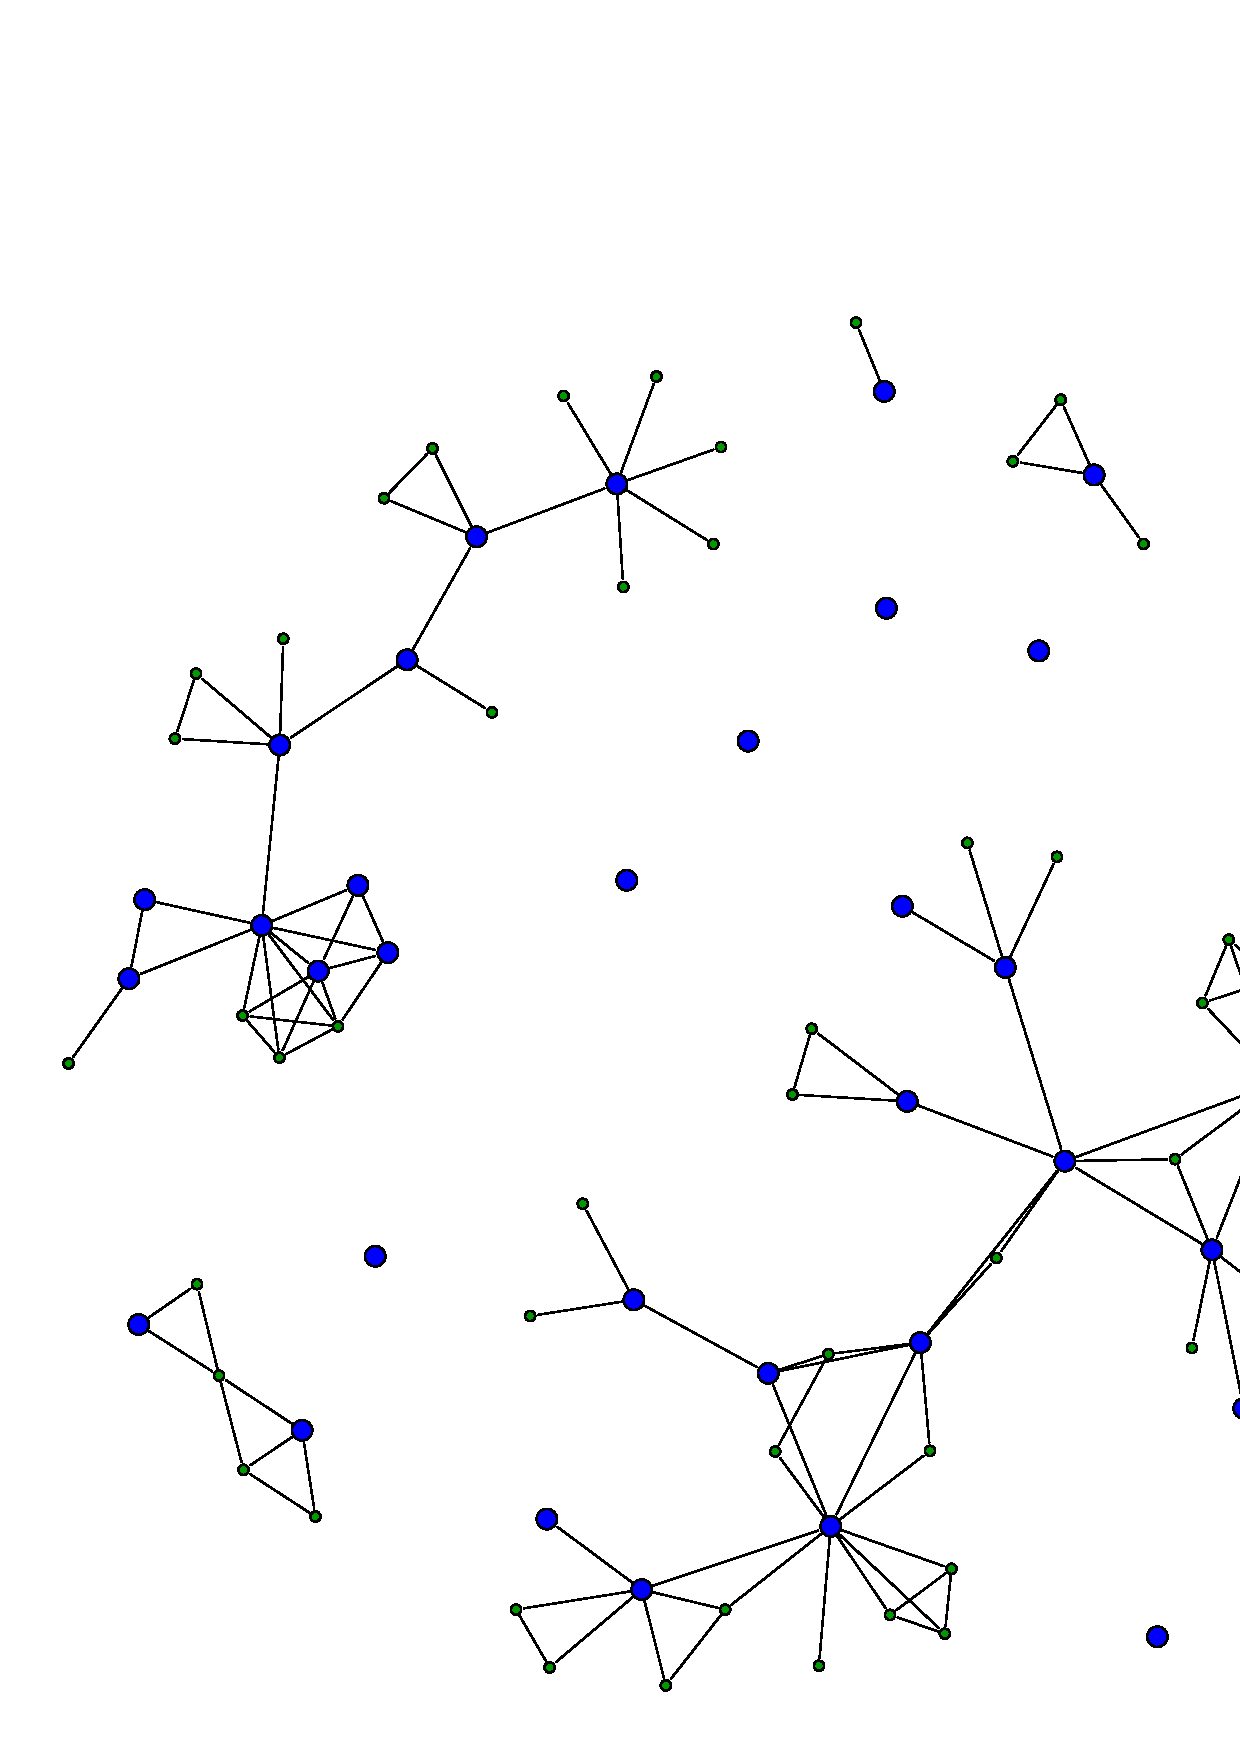
\includegraphics[width=5cm]{figuras/graph}
%\caption{\label{fig:graph}Exemplo de uma figura.}
%\end{figure}
\chapter{Desenhando objetos}
\label{cap:desenvolvimentos}
% O objetivo deste cap�tulo � expor as t�cnicas e decis�es para gerar as imagens das cartas no
% celular

% Introduzir aos conceitos b�sicos de imagens, perspectiva, vis�o e objetos em rela��o � conputa��o
% gr�fica, as tecnologias como biblioteca gr�fica e bibliotecas do android para desenvolvimento de
% aplicativos

% Explicar as decis�es tomadas no desenvolvimento do GL(biblioteca gr�fica no aplicativo). Explicar
% as abstra��es que foram feitas para obter o GL.

% Mostras testes de experimento de tempo durante o processo de otimiza��o.

O Android pode ser visto como uma camada de abstra��o da interface de manipula��o da tela do celular e
do sensor de toque da tela disponibilisados pelos fabricantes. Nosso aplicativo faz uso desses
dispositivos, por meio desta camada e n�o iremos nos preocupar como essa abstra��o foi implementada.

O OpengGL ES � um conjunto de comandos que permitem a especifica��o de objetos geom�tricos em duas
ou tr�s dimen��es, junto com comandos que controlam como esses objetos s�o renderizados no
framebuffer.

Desta forma iremos usar o OpengGL para gerar o que deve ser desenhado na tela e faremos uso dos
m�todos e classes do android para expor a imagem na tela e receber informa��es sobre eventos de toque.